\documentclass[aspectratio=169,11pt]{beamer}
\usepackage[T1]{fontenc}\usepackage{lmodern,graphicx,booktabs}
\definecolor{navy}{HTML}{18364A}\definecolor{teal}{HTML}{008B80}
\setbeamercolor{normal text}{fg=navy,bg=white}\setbeamercolor{frametitle}{fg=navy}\setbeamercolor{structure}{fg=teal}
\setbeamerfont{frametitle}{size=\Large,series=\bfseries}
\setbeamertemplate{navigation symbols}{}
\setbeamertemplate{footline}{}
\setbeamercolor{block title}{fg=white,bg=teal}
\setbeamercolor{block body}{fg=navy,bg=teal!7}
\setbeamersize{text margin left=7mm,text margin right=7mm}
\begin{document}
\begingroup\setbeamercolor{background canvas}{bg=navy}\begin{frame}[plain]\color{white}
{\small CISC 473 $\cdot$ Group 04}\par\vspace{6mm}{\Huge\bfseries Where to adapt BART?}\par\vspace{4mm}Does the location of a LoRA adapter change summary quality when the parameter budget stays fixed?\par\vspace{6mm} Choo Wen Bin and Nai Junn Rong\end{frame}\endgroup
\begin{frame}{Three ideas motivate the comparison}
\begin{itemize}
\item BART: a pretrained encoder--decoder for conditional generation
\item LoRA and Prefix-Tuning: different ways to adapt frozen weights
\item AdaLoRA / DyLoRA / WeightLoRA: allocation and rank matter
\item FactCC: word overlap is not factual support
\item Our contribution: a controlled architectural comparison
\end{itemize}
\end{frame}
\begin{frame}{Three locations, three computational roles}\begin{columns}[T,onlytextwidth]\column{.315\linewidth}\begin{block}{Encoder self-attention}Builds a representation of the source article.\end{block}\column{.315\linewidth}\begin{block}{Decoder self-attention}Tracks the summary generated so far.\end{block}\column{.315\linewidth}\begin{block}{Cross-attention}Connects the next word in the summary to the source article.\end{block}\end{columns}\vspace{6mm}\par BART-base: 6 encoder layers, 6 decoder layers, width 768.\end{frame}
\begin{frame}{Match capacity before comparing placement}
\begin{itemize}
\item W = W$_0$ + ($\alpha$/r)BA; the backbone stays frozen
\item Rank r = 8; $\alpha$ = 16; adapter dropout = 0.05
\item Query and value projections in six blocks
\item 6 $\times$ 2 $\times$ 8 $\times$ (768 + 768) = 147,456 trainable parameters
\item Exactly the same budget for all three main placements
\end{itemize}
\end{frame}
\begin{frame}{Fixed subsets, separate held-out tests}
\begin{itemize}
\item CNN/DailyMail: 1,024 train / 64 validation / 128 test
\item XSum: 128 test examples; no further training
\item Subset seed 42; training seeds 42, 123 and 999
\item Source limit 1,024 tokens; training target limit 128
\item ROUGE uses original, untruncated reference summaries
\end{itemize}
\end{frame}
\begin{frame}{Training effort is controlled, with one exception}
\begin{itemize}
\item 3 epochs = 96 updates; effective batch size 32
\item AdamW; PEFT learning rate 3$\times$10$^{-4}$; full FT 3$\times$10$^{-5}$
\item Main runs: microbatch 2 $\times$ accumulation 16
\item Full FT retry: microbatch 1 $\times$ accumulation 32 after memory failure
\item Equal updates do not mean equal FLOPs or wall-clock time
\end{itemize}
\end{frame}
\begin{frame}{Evaluate generated summaries, not loss alone}
\begin{itemize}
\item ROUGE-1 / ROUGE-2 / ROUGE-L: stemmed macro F1 $\times$ 100
\item Four-beam decoding; lengths 56--128; no repeated trigrams
\item Final-epoch checkpoint; no test-based checkpoint selection
\item Mean $\pm$ sample SD over 3 training seeds
\item Seed SD is not a confidence interval over articles
\end{itemize}
\end{frame}
\begin{frame}{The completed experiment matrix}
\begin{itemize}
\item 3 isolated placements + unadapted BART
\item All-attention QV ranks 4, 8 and 16
\item All-attention Q-only, K-only, V-only and QKVO
\item Prefix-Tuning and full fine-tuning
\item 13 configurations $\times$ 3 seed labels $\times$ 2 test datasets = 78 evaluations
\end{itemize}
\end{frame}
\begin{frame}{Cross-attention leads the matched placements}
\begin{center}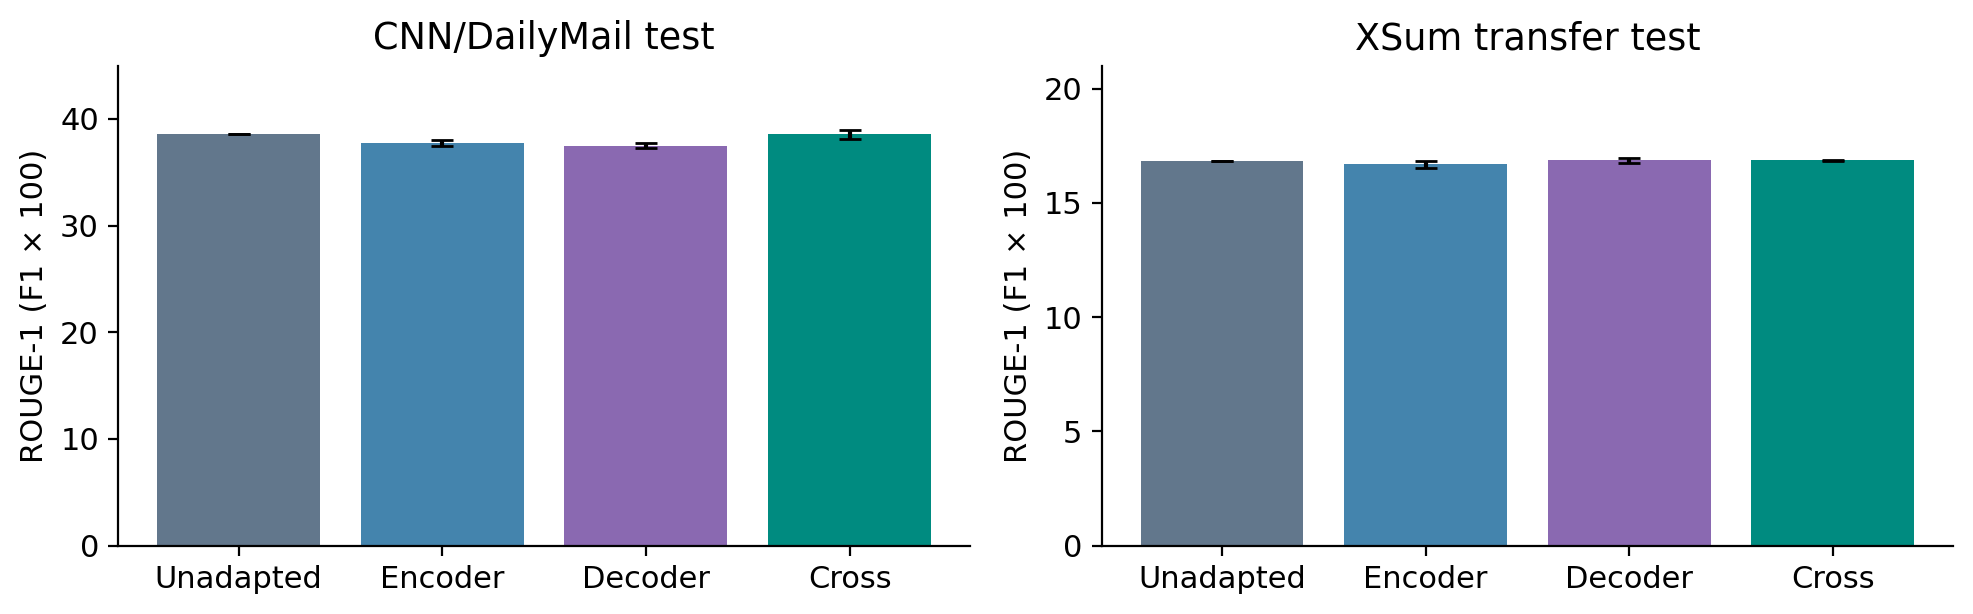
\includegraphics[width=.88\linewidth,height=.49\textheight,keepaspectratio]{figures/placement.png}\end{center}
\begin{itemize}
\small
\item CNN/DailyMail R-1: cross 38.56; encoder 37.75; decoder 37.50
\item Unadapted R-1: 38.61; cross does not improve this baseline
\item XSum placement R-1 means are close: 16.68--16.87
\end{itemize}
\end{frame}
\begin{frame}{Full FT is strongest; Prefix struggles here}
\begin{center}\begin{tabular}{lrr}\toprule Configuration & CNN R-1 & XSum R-1\\\midrule
Unadapted & 38.61 $\pm$ 0.00 & 16.84 $\pm$ 0.00\\
Cross-attention & 38.56 $\pm$ 0.42 & 16.87 $\pm$ 0.02\\
All-attention QV & 38.92 $\pm$ 0.08 & 17.16 $\pm$ 0.09\\
Prefix & 15.05 $\pm$ 3.03 & 9.75 $\pm$ 1.71\\
Full FT* & 40.06 $\pm$ 0.62 & 19.17 $\pm$ 0.23\\
\bottomrule\end{tabular}\end{center}
\begin{itemize}
\small
\item Full FT has the highest baseline mean ROUGE-1 on both subsets
\item All-attention QV uses 442,368 parameters: 3$\times$ the isolated budget
\item Prefix results describe this short-budget implementation
\item Full FT* remains a memory-adjusted reference
\end{itemize}
\end{frame}
\begin{frame}{More parameters do not guarantee higher ROUGE}
\begin{center}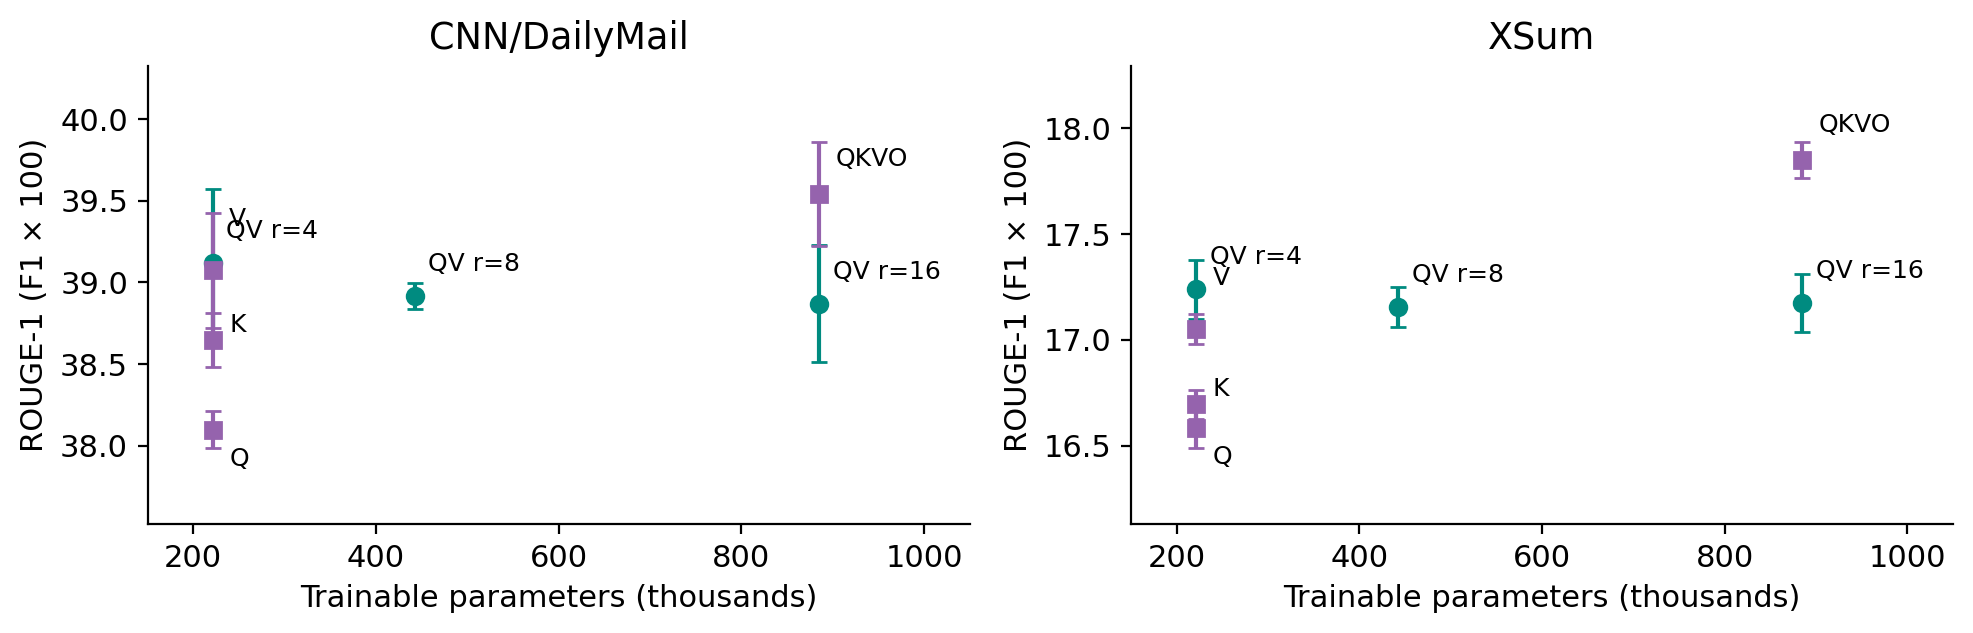
\includegraphics[width=.88\linewidth,height=.49\textheight,keepaspectratio]{figures/ablations.png}\end{center}
\begin{itemize}
\small
\item QV rank 4 $\rightarrow$ 8 $\rightarrow$ 16 does not give monotonic gains
\item Rank sweep keeps $\alpha$ = 16, so $\alpha$/r also changes
\item V-only has the strongest single-projection R-1 means
\item QKVO has the strongest LoRA R-1 means, at a larger budget
\end{itemize}
\end{frame}
\begin{frame}{Parameter efficiency and runtime are different}
\begin{itemize}
\item All isolated placements: exactly 147,456 trainable parameters
\item Encoder training loop: 2.31 $\pm$ 0.07 h
\item Decoder: 1.42 $\pm$ 0.02 h; cross-attention: 1.39 $\pm$ 0.03 h
\item Times include epoch validation and checkpoint saving
\item Frozen backbone weights and activations still consume memory
\end{itemize}
\end{frame}
\begin{frame}{Human ratings: descriptive, with low agreement}
\begin{center}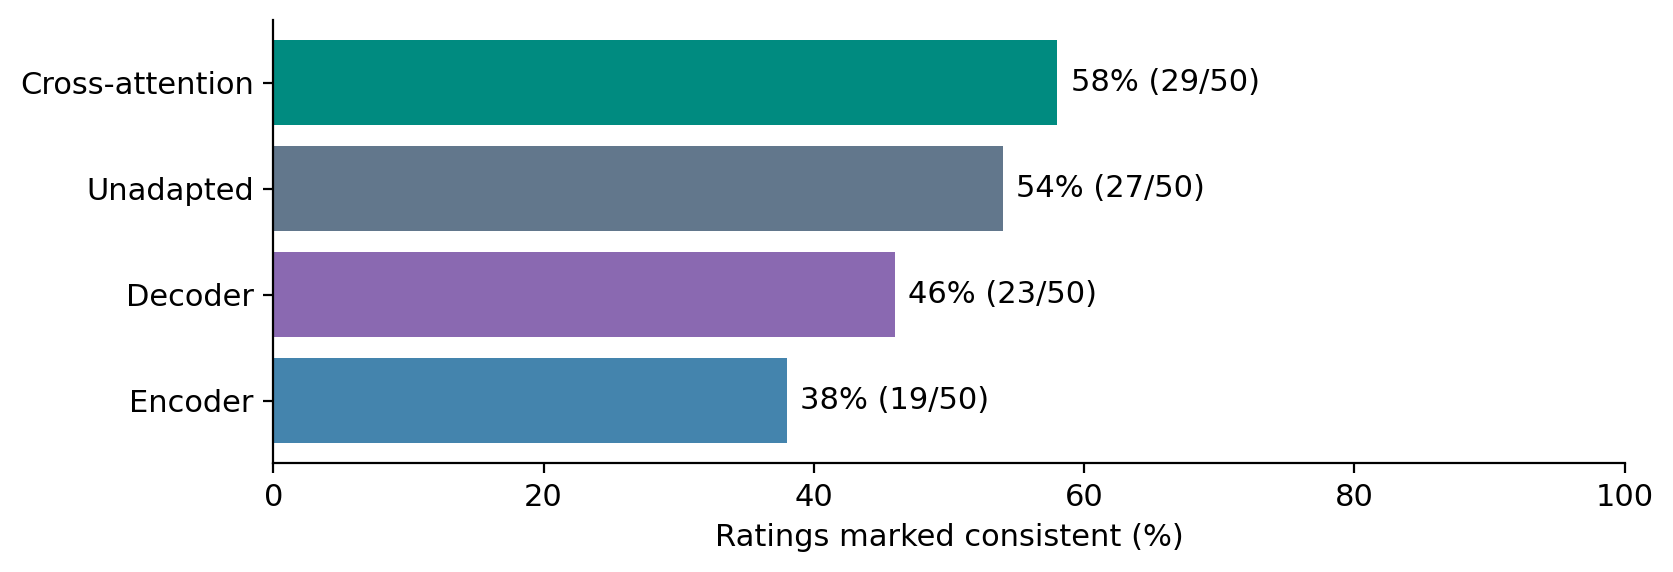
\includegraphics[width=.88\linewidth,height=.49\textheight,keepaspectratio]{figures/human.png}\end{center}
\begin{itemize}
\small
\item 10 people $\times$ 20 outputs = 200 ratings
\item 5 articles $\times$ 4 configurations; seed 42; randomized blind order
\item Pairwise agreement 52.22\%; Fleiss' $\kappa$ = 0.044
\item 200 ratings are not 200 independent articles
\end{itemize}
\end{frame}
\begin{frame}{A concrete factual failure}
\begin{itemize}
\item Source: Aaron Cook is 24 and has received a Moldovan passport
\item Encoder output: ``The 31-year-old has been granted citizenship…''
\item Later: ``…has been denied citizenship by the Republic of Moldova.''
\item Age error + polarity reversal + internal contradiction
\item All 10 raters marked this output inconsistent; one illustrative case
\end{itemize}
\end{frame}
\begin{frame}{What we can and cannot conclude}
\begin{itemize}
\item Cross-attention leads isolated placements on in-domain ROUGE means
\item No clear R-1 improvement over unadapted BART; no factuality winner
\item Small fixed subsets; 96 updates; one backbone
\item Full FT microbatch exception; unequal wall time / FLOPs
\item XSum length policy and low rater agreement limit interpretation
\end{itemize}
\end{frame}
\begin{frame}{Conclusion and next experiment}
\begin{itemize}
\item Placement affects observed quality under an exact adapter budget
\item Broader coverage helps R-1 here, but uses more parameters
\item Next: larger fixed-data study + paired article-level uncertainty
\item Prior team declaration: Wen Bin 50\%; Junn Rong 50\%
\item AI disclosure: OpenAI Codex and academic-humanizer assisted this work
\end{itemize}
\end{frame}
\begin{frame}{References: methods}\small\begin{itemize}
\item Lewis et al. (2020). BART. ACL, 7871--7880.
\item Hu et al. (2022). LoRA. ICLR. arXiv:2106.09685.
\item Li and Liang (2021). Prefix-Tuning. ACL-IJCNLP, 4582--4597.
\item Zhang et al. (2023). Adaptive Budget Allocation for PEFT. ICLR.
\item He et al. (2022). Towards a Unified View of PEFT. ICLR.
\item Valipour et al. (2023). DyLoRA. EACL, 3274--3287.
\item Veprikov et al. (2026). WeightLoRA. ACL. Entry from supplied midterm.
\end{itemize}\end{frame}
\begin{frame}{References: evaluation, data and tools}\small\begin{itemize}
\item Kryscinski et al. (2020). Evaluating Factual Consistency. EMNLP, 9332--9346.
\item Lin (2004). ROUGE: A Package for Automatic Evaluation of Summaries.
\item Model: facebook/bart-base; data: abisee/cnn\_dailymail 3.0.0 and EdinburghNLP/xsum.
\item PyTorch 2.5.1+cpu; Transformers 4.44.2; PEFT 0.13.2; Evaluate 0.4.3.
\item Code: github.com/wenbin05/DeepLearningP08. Revisions and protocol: report appendix.
\item AI assistance: OpenAI Codex; academic-humanizer skill. Human ratings: team-supplied.
\item Primary literature pages could not be re-fetched here; verify citations before submission.
\end{itemize}\end{frame}
\end{document}
